\documentclass{beamer}
\usepackage{amsmath}
\usepackage[utf8]{inputenc}
\usepackage{graphicx}
\usetheme{Warsaw}
\usecolortheme{wolverine}
\DeclareMathOperator{\taninv}{tan^{-1}}


\title{EE2227 CONTROL SYSTEMS PRESENTATION}
\author{ADITYA PEDAVEGI\\EE18BTECH11034}
\begin{document}
\maketitle
\begin{frame}{GATE ECE 2016 Q.No:20}
The number of directions and encirclements around the point -1+j0 in the complex plane by the Nyquist plot of $$G(s) = \frac{1-s}{4+2s}$$

\bigskip
\begin{itemize}
    \item Zero
    \item One, Anti-Clock wise
    \item One, Clock wise
    \item Two, Clock wise
\end{itemize}
\end{frame}

\begin{frame}{Solution}

First,we need to draw the polar plot of given G(S).
In the polar plot,substitute s = j\omega
\\
$$ G(j\omega) = \frac{1-j\omega}{4+2j\omega} $$
\\
$$ \lim_{\omega\to\infty} G(j\omega) = \frac{1-j\omega}{4+2j\omega} $$
\\
$$ \lim_{\omega\to\infty} G(j\omega) = \frac{j\omega(\frac{1}{j\omega}-1)}{j\omega(\frac{4}{j\omega}+2)} $$ 
\\
$$ \lim_{\omega\to\infty} G(j\omega) = \frac{-1}{2}\angle 0 $$ 
\\

\centering which is equal to $\frac{1}{2}\angle{-180}$
\end{frame}

\begin{frame}
As the Magnitude is taken positive in Nyquist Plot.\\
Now substitute \omega = 0
\\
$$ \lim_{\omega\to\ 0} G(j\omega) = \frac{1-j\omega}{4+2j\omega} = \frac{1}{4}\angle 0 $$

$$\angle Num(G(j\omega)) = \taninv \frac{-\omega}{1} = -\taninv \frac{\omega}{1}$$
\\
$$\angle Den(G(j\omega)) = \taninv \frac{\omega}{2} = \taninv \frac{\omega}{2}$$
\\
\angle $G(j\omega) = \angle Num(G(j\omega)) - \angle Den(G(j\omega))$

\bigskip
so from this  at $\omega = 0$ \angle $G(j\omega) = 0$

\bigskip
and so from this  at $\omega = $\infty$ \angle $G(j\omega)  =$-\pi$     
\end{frame}

\begin{frame}
$$ \mid(G(j\omega))\mid = \frac{\sqrt{1+{\omega}^2}}{\sqrt{16+{4\omega}^2}} $$
\\
when $\omega =0$ \mid(G(j\omega))\mid = \frac{1}{4}
\bigskip
\\

when $\omega = \infty$ \mid(G(j\omega))\mid = \frac{1}{2}
\bigskip
\\
Hence,magnitude should be every time positive.
\\
So,we have to plot first 0.25 then we have to turn {-180} degrees to that point i.e {180} degrees clockwise(in this case)

\end{frame}
\begin{frame}
\begin{itemize}
\item Now Plot the Polar Plot 1 from $\omega$=0 to $\infty$
\\

$$ 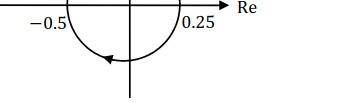
\includegraphics[scale = 0.5]{image2.jpg}$$
\\
\item Draw the Mirror image of the Polar Plot 1.
\\
$$ 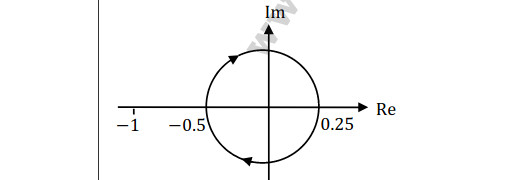
\includegraphics[scale = 0.5]{image1.jpg}$$
\\
\item Find the points where $G(j\omega)$ intersects the real and imaginary axes(if needed) and then locate the given co-ordinate
\end{itemize}
\\
\bigskip
\end{frame}

\begin{frame}{Nyquist plotting}
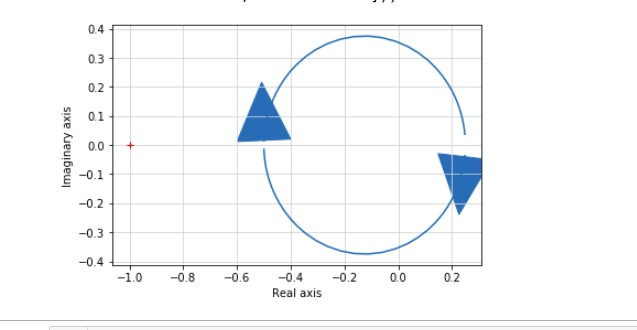
\includegraphics[scale = 0.5]{python nyquist plot.jpg}
\end{frame}

\begin{frame}
    $$Put\,s=Re^{j\theta}$$
    $$\lim_{R\to \infty}\,G(Re^{j\theta})=\frac{1-Re^{j\theta}}{4+2Re^{j\theta}}=\frac{-1}{2}$$ \\
    \bigskip
    As there are no $e^{j\theta}$ terms, 
    \\
    There there will be no enclosed Nyquist path here. 
    \\
    So, for this Transfer function $G(s)$,the Nyquist plot is same as the Polar plot.
    
\end{frame}

\begin{frame}
As from the observed plot the co-ordinate -1 + j0 is outside the contour
\\
\bigskip
\\
Hence,the number of encirclements around the the given co-ordinate is zero.
\end{frame}

\end{document}

